\documentclass{article}
\usepackage{tikz}
\usetikzlibrary{arrows.meta}

\begin{document}

\begin{figure}[h]
\centering
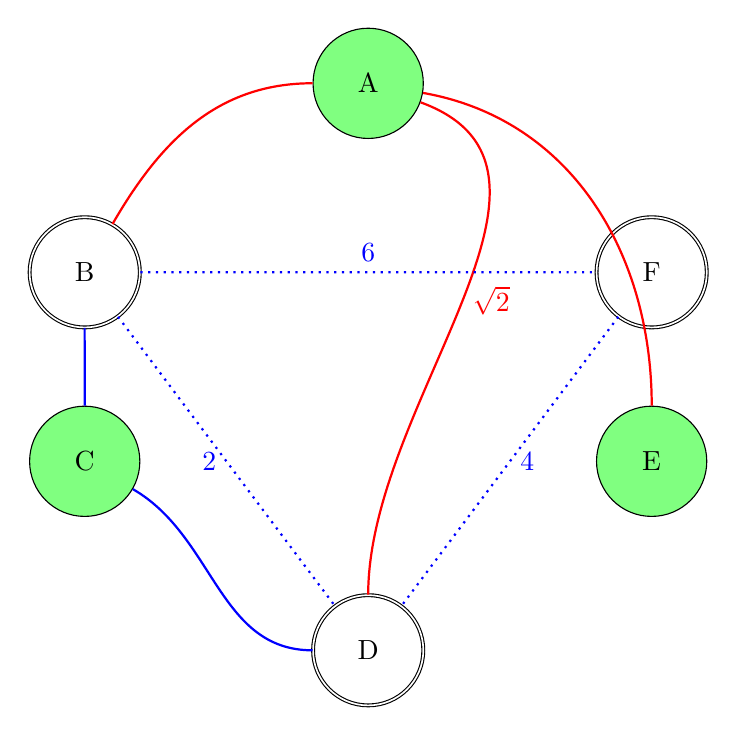
\begin{tikzpicture}[scale=1.2]

\node[circle, draw, fill=green!50, minimum size=14mm] (A) at (0,4) {A};

\node[circle, double, draw, minimum size=14mm] (B) at (-3,2) {B};
\node[circle, double, draw, minimum size=14mm] (F) at (3,2) {F};

\node[circle, draw, fill=green!50, minimum size=14mm] (C) at (-3,0) {C};
\node[circle, draw, fill=green!50, minimum size=14mm] (E) at (3,0) {E};

\node[circle, double, draw, minimum size=14mm] (D) at (0,-2) {D};

\draw[red, thick]
  (B) to[out=60, in=180] (A);

\draw[red, thick]
  (A) to[out=-20, in=90]
  node[midway, right, red] {$\sqrt{2}$} (D);

\draw[red, thick]
  (A) to[out=-10, in=90] (E);

\draw[blue, thick, dotted]
  (B) -- node[midway, above, blue] {$6$} (F);

\draw[blue, thick, dotted]
  (B) -- node[midway, left, blue] {$2$} (D);

\draw[blue, thick, dotted]
  (F) -- node[midway, right, blue] {$4$} (D);

\draw[blue, thick]
  (B) -- (C);

\draw[blue, thick]
  (C) to[out=-30, in=180] (D);

\end{tikzpicture}
\end{figure}

\end{document}
